\section{Stairway to Heaven}

\subsection{Problem}

You want to reach the heaven, which is at the top of a staircase. The staircase has $n$ steps. At each step, you can climb either one step or two steps further. In how many ways can you reach heaven?

\begin{figure}[H]
    \centering
    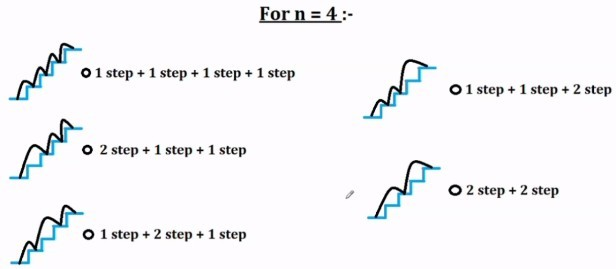
\includegraphics[width=0.6\textwidth]{./images/stairway_to_heaven_0.jpg}
    \caption{Example of all possible ways for n = 4}
\end{figure}

\subsection{Solution - Recursion}

Let $W$ be the function which associates a number of steps with the number of \textbf{W}ays you can reach heaven.

\begin{algorithm}[H]
    \caption{Opt}
    \label{stairway-to-heaven:algorithm:naive}
    \begin{algorithmic}[1]
        \State{W(n) = W(n - 1) + W(n - 2)}
        \State{W(0) = 1}
        \Comment{if you are already there, then there is one way, stay where you are}
        \State{W(1) = 1}
        \State{W(2) = 2}
    \end{algorithmic}
\end{algorithm}

Such solution allows memoization.

\subsection{Solution - Sum}

\begin{algorithm}[H]
    \caption{Opt}
    \label{stairway-to-heaven:algorithm:opt}
    \begin{algorithmic}[1]
        \State{limit = quotient(n, 2)}
        \State{W(n) = $\sum\limits_{i = 0}^{limit} \dfrac{(n-i)!}{i! (n - 2i)!}$}
    \end{algorithmic}
\end{algorithm}

That is not particularly obvious, but if you spend some time analysing how one constructs all possibilities and if you apply a bit of combinatorial analysis, you get there...

\subsection{Solution - Fibonacci}

Notice that the solution to this problem is a Fibonacci number.
